% !TEX encoding = UTF-8
% !TEX TS-program = pdflatex
% !TEX root = ../tesi.tex

%**************************************************************
\chapter{Our work}
\label{cap:progettazione-codifica}
%**************************************************************

\intro{In this chapter we present what we did. In section \ref{sec:pre} we present the preprocessing of the logs and in section \ref{sec:exp} we cover the experiments we performed.}

%**************************************************************

\section{\label{sec:pre}Preprocessing}

	\subsection{Data cleaning}
		The first thing we did was cleaning the data. 
		This operation was necessary because the parser parsed also the prematch. 
		This part of the game would have been a problem because the players usually do not move and the vision does not move even if the player moves the mouse. 
		Moreover, there is some time, during which the players cannot move.
		That would result in any player stopping for the prematch's amount of time.
		This caused the necessity to clean the data to remove the prematch from the parsed log.
	
	\subsection{\label{sec:cut}Match cutting}
		Given that the matches can be very long and that can have different durations, we decided to cut them and keep only the first ten minutes of every game. 
		It was easy to understand where to cut the file because the parser we used wrote, in every line, the corresponding \gls{tick}. 
		Knowing how many ticks per second there are in the game, we were able to calculate how many ticks we had to keep in the log and cut the file accordingly.
		
	\subsection{Sequence creation}
		We had 100 matches for each player, and after cutting them, we had only the first ten minutes of every game. 
		In our task, the less time we need for reliable identification, the better. 
		So we decided to divide each log into 5 parts, each one corresponding to a sequence of two minutes of gameplay. 
		To achieve this, we used the same method described in \ref{sec:cut}, using the ticks as guidelines. 
		
	\subsection{Interpolation}
		
		We noticed that the parser had a problem concerning the creation of the logs. 
		The logs are made of dumps that occur every two ticks. 
		Sometimes, though, there were some missing ticks.
		We had to find a way to deal with the missing data. 
		Given that the missing data were not many, we decided to interpolate them.
		This solution is widely used to deal with missing data in sequences and allows to keep the behaviours if the missing data are a few compared to the entire sequence, and that happened to be our case. 
		If there was only one tick to be interpolated, so there was a four ticks difference between two lines, the interpolation was done computing the mean of the previous and the successive tick. 
		In case there were multiple missing ticks, we chose to interpolate in the same way. 
		That has the effect of making it look like the player exponentially slows down the movement. 
		We thought this could be a plausible behaviour, mainly because the player's motions try to be as precise as possible, so the players may slow down the movement when they comes close to their objective.
	
	\subsection{Data aggregation}
		
		The following step is data aggregation. 
		A crucial decision is how many ticks to aggregate. 
		With DOTA 2, the decision was to aggregate 15 ticks. 
		This decision resulted in aggregating portions of gameplay with a duration of half a second. In our work, we did some experiments to understand which one was the best option. 
		In CS:GO, there are 64 ticks in a second, so we tried to aggregate 16 and 32 ticks, corresponding respectively to a quarter and half a second. 
		In the following images, some graphs can help to understand the difference between the two options. 
		The first graph, in Figure \ref{fig:gr0}, shows the trend of the player's speed along the z-axis, of one of the matches.
		
		\begin{figure}[!h] 
			\centering 
			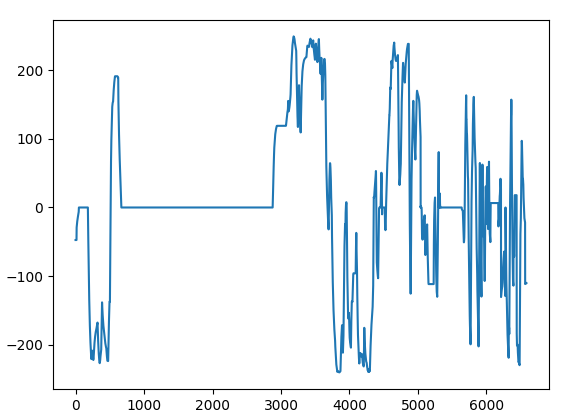
\includegraphics[scale=.7]{grafici/Grafico 2.png}
			\caption{\label{fig:gr0}Graph of the player's speed along the z axis.}
		\end{figure}
		
		In figure \ref{fig:gr1}, we can see the same data. 
		The only difference is that the second image presents the log after the aggregation process occurred.
		This graph shows the result of the trend after a 16-ticks-aggregation. 
		In figure \ref{fig:gr2}, we can see the same chart after a 32-ticks-aggregation. 
		
		\begin{figure}[!h] 
			\centering 
			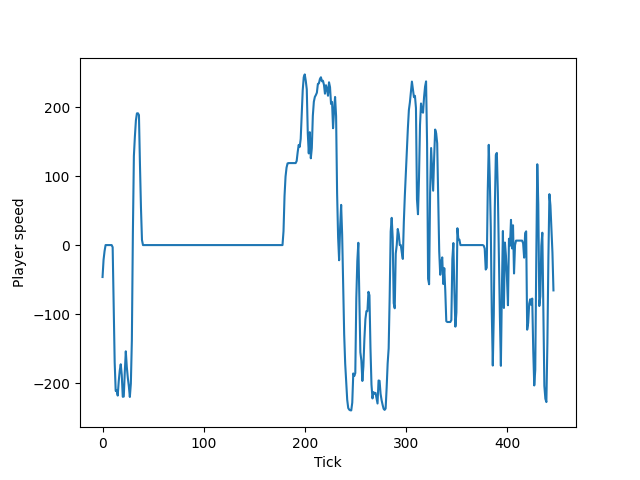
\includegraphics[scale=.7]{grafici/Grafico 3.png}
			\caption{\label{fig:gr1}Graph of the player's speed along the z axis after a 16-ticks aggregation.}
		\end{figure}
		
		\begin{figure}[!h] 
			\centering 
			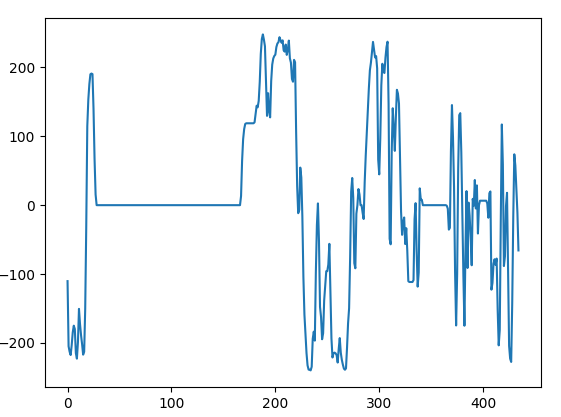
\includegraphics[scale=.7]{grafici/Grafico 4.png}
			\caption{\label{fig:gr2}Graph of the player's speed along the z axis after 32-ticks aggregation.}
		\end{figure}
		
		As shown in the previous images, there is a difference in aggregating with 16 or 32 ticks. 
		Of course, the graph shows only one data sequence, but we did not base our decision only on the information we could retrieve from this single graph. 
		The decision was taken after studying the differences in distributions of the values to identify the best number of ticks to aggregate, 
		using the Kolmagorov-Smirnov statistics to quantify the distance between the raw data and the aggregated data, as shown in Quantifying Information Loss Through Data Aggregation~\cite{womak:info_loss}.
		The candidate values were $16$ and $32$, because any number lower than $16$ would have been not enough to reduce memory usage and any number higher than $32$ would result in losing too much information. 
		After evaluating both the candidate values, although the difference is not very big, we decided it would have been better to use the 16-ticks-aggregation because it results in a lower information loss. 
		
		
	\subsection{Split creation}
	
		The following step was to split the dataset into three sets: the training set, the validation set, and the test set. 
		We decided to use an 80\%-10\%-10\% split. 
		The dataset was split as part of the preprocessing to avoid the model using the test set in some of the epochs as part of the training and to avoid computing a split every time we ran the neural network training script.
		
	\subsection{Standardization}

		To save time in the training process, we decided to standardize all the logs as part of the preprocessing phase. We decided to use the standard scaler provided by sklearn\footnote{\href{https://scikit-learn.org/stable/modules/generated/sklearn.preprocessing.StandardScaler.html}{https://scikit-learn.org/stable/modules/generated/sklearn.preprocessing.StandardScaler.html}}. 
		This scaler needs to be fit on the data, and we decided to do so using the training split. 
		The result is that the training split was scaled in the range $[-1, 1]$, while the validation and test split were scaled but not necessarily in the $[-1, 1]$ range. 
		This decision was taken to avoid overfitting problems, due to the fact that we do not know what data we can find in the validation or test set.

%**************************************************************

\section{\label{sec:exp}Experiments}

	\subsection{First model}
			
		In our work, just as DOTA 2, we decided to use a Recurrent Neural Network, specifically a Long Short Term Memory (LSTM). 
		This decision was almost mandatory because we worked with sequences and because the time information is relevant. 
		LSTM is, in fact, a type of neural network in which information persists in time. 
		For instance, an LSTM neural network can learn the pattern followed by a specific player in the movements on the map, while a simple neural network cannot.
		Following the same intuition behind the DOTA 2 work, we thought that some actions, such as the camera movements, can be biometric, meaning that everyone has a different way to do it.\\
		
		
		In our model, there are two LSTM layers with $\tanh$ activation function, a fully connected layer with $RELU$ activation  function, and a $softmax$ output layer.
		%In the final model there are also two Dropouts layer, with a $0.2$ rate, one after each LSTM layer, even though they were not present in the first model we used.
		The LSTM layers have 256 units each, while the first fully connected layer has 128 units. 
		The output layer has 50 units, due to the number of classes we had. 
		We used a batch size of 128, 100 epochs of training, and the categorical crossentropy loss function. 
		The optimizer we chose is Adam, with a learning rate of $0.01$. 
		Figure \ref{fig:mod1} shows a summary of our model. 
		For the implementation, we used the Keras\footnote{\href{https://keras.io/}{https://keras.io/}} library with a Tensorflow\footnote{\href{https://www.tensorflow.org/}{https://www.tensorflow.org/}} backend. 
		The GPU we used is an Nvidia GeForce GTX 1050 2Gb.
		
		\begin{figure}[!h] 
			\centering 
			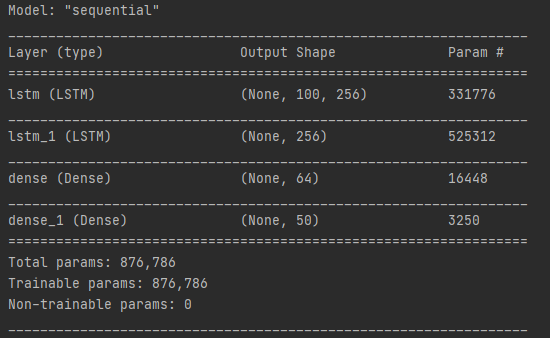
\includegraphics[scale=.6]{modelli/primo_modello.png}
			\caption{\label{fig:mod1}Summary of the first model used.}
		\end{figure}
		
		This first model reached $\sim 0.8$ accuracy and $\sim 0.75$ precision on the validation set. 
		
	\subsection{Feature selection}
	
		The first model we coded had surprisingly high accuracy and precision. 
		Then we tried to eliminate a set of features so that the model could learn better. 
		We used our intuition to identify some features that could introduce noise in the predictions. 
		We thought that the mean of the position on the map could introduce some noise since it depends on the map chosen for the match. 
		Speaking of actions, we noticed that some of the parsed actions were never triggered and, after some researches, we found that the game itself never triggered such events. 
		Given the situation, we decided to ignore these actions, such as the action $door\_moving$. 
		In Table \ref{tab:features} there is a list of the features we kept. 
		
		\begin{longtable}{|c|c|}

			\caption{\label{tab:features}Features we kept after the feature selection process}

			\hline
			\textbf{Type} & \textbf{Features} \\
			\hline
			Mouse position (x axis) & Mean, standard deviation, changes in positive, changes in negative\\
			\hline
			Mouse position (y axis) & Mean, standard deviation, changes in positive, changes in negative\\
			\hline
			Player position (x axis) & Standard deviation, changes in positive, changes in negative\\
			\hline
			Player position (y axis) & Standard deviation, changes in positive, changes in negative\\
			\hline
			Player position (z axis) & Standard deviation, changes in positive, changes in negative\\
			\hline
			Player velocity (x axis) & Mean, standard deviation, changes in positive, changes in negative\\
			\hline
			Player velocity (y axis) & Mean, standard deviation, changes in positive, changes in negative\\
			\hline
			Player velocity (z axis) & Mean, standard deviation, changes in positive, changes in negative\\
			\hline
			Crouch changes & n\_occurs\\
			\hline
			Weapon fire & n\_occurs \\
			\hline
			Weapon reload & n\_occurs \\
			\hline
			Player jump & n\_occurs \\
			\hline
			Kills & n\_occurs \\
			\hline
			Assists & n\_occurs \\
			\hline
			Item pickup & n\_occurs \\
			\hline
			Item equip & n\_occurs \\
			\hline
			Grenade detonate  & n\_occurs \\
			\hline
			Smokegrenade detonate & n\_occurs \\
			\hline
			Molotov detonate & n\_occurs \\
			\hline
			Flashbang detonate & n\_occurs \\
			\hline
			Tagranade detonatoe & n\_occurs \\
			\hline
			Hegranade detonate & n\_occurs \\
			\hline
			Decoy detonate & n\_occurs \\
			\hline
			Player falldamage & n\_occurs \\
			\hline
			Ammo pickup & n\_occurs \\
			\hline
			Silencer detach & n\_occurs \\
			\hline
		\end{longtable}
	
	\subsection{Model selection}
	
		The following runs of the training script resulted in a better-performing neural network. 
		We could easily reach 90\% accuracy and precision in both the validation and test set, as shown in figures \ref{fig:acc1} and \ref{fig:acc2}.
		We were also able to stabilize the loss as shown in Figure \ref{fig:loss1} and \ref{fig:loss2}.
		
		\begin{figure}[!h]
			\centering
			\begin{minipage}{.5\textwidth}
				\centering
				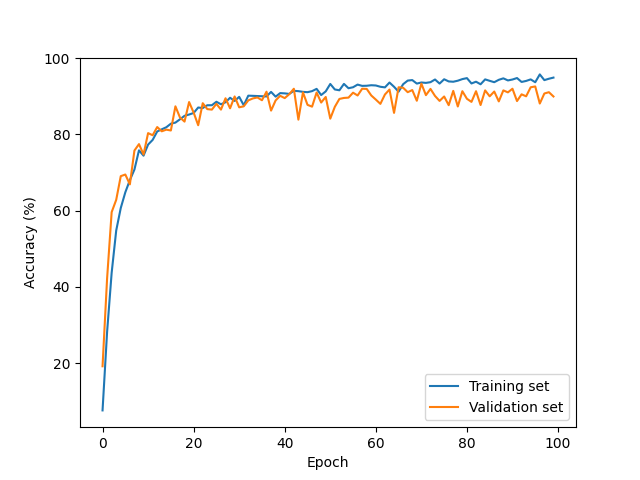
\includegraphics[width=.8\linewidth]{risultati/accuracy.png}
				\caption{\label{fig:acc1}Training and \\ validation accuracy}
			\end{minipage}%
			\begin{minipage}{.5\textwidth}
				\centering
				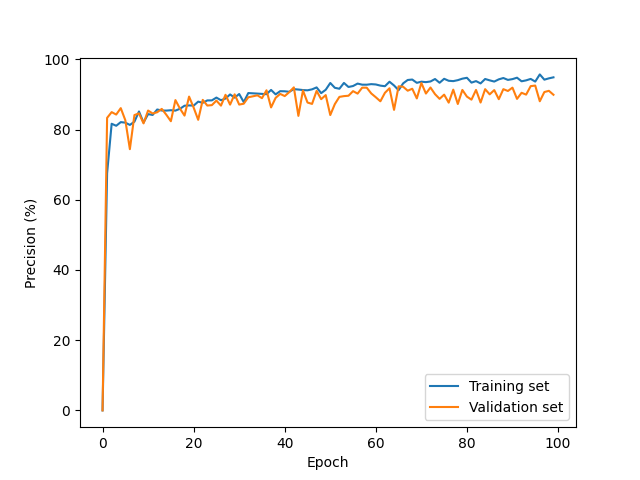
\includegraphics[width=.8\linewidth]{risultati/precision.png}
				\caption{\label{fig:acc2}Training and \\ validation precision}
			\end{minipage}
		\end{figure}
		
		\begin{figure}[!h]
			\centering
			\begin{minipage}{.5\textwidth}
				\centering
				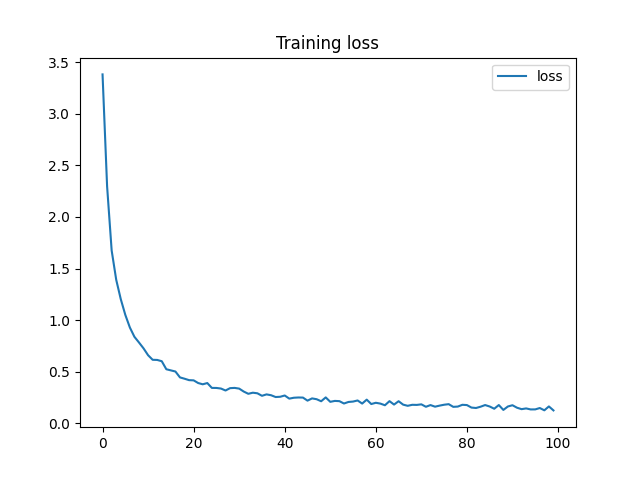
\includegraphics[width=.8\linewidth]{risultati/train_loss.png}
				\caption{\label{fig:loss1}Training loss}
			\end{minipage}%
			\begin{minipage}{.5\textwidth}
				\centering
				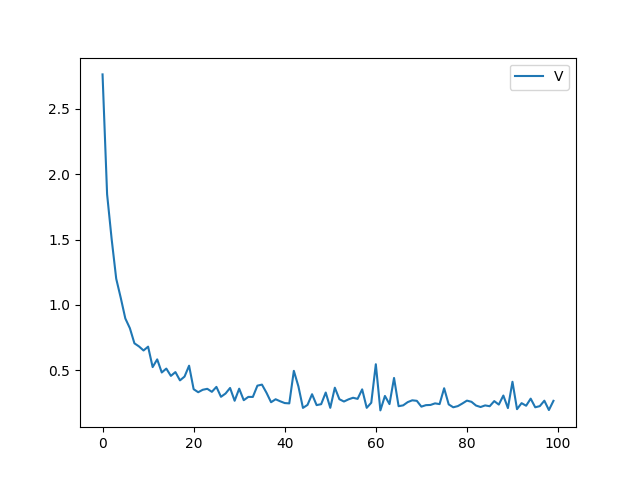
\includegraphics[width=.8\linewidth]{risultati/val_loss.png}
				\caption{\label{fig:loss2}Validation loss}
			\end{minipage}
		\end{figure}
		
		During the experiments phase, we tried some different solutions. 
		Due to the short time we had, though, we could not experiment a lot. 
		The first thing we tried was changing the optimizer's learning rate parameter. 
		The values we used were $0.01$, $0.001$, and $0.0001$. 
		The result was that the best learning rate was, considering the loss value, $0.0001$, even if the difference between that and $0.001$ was very little. 
		Then we tried to understand if the decay had a positive influence on the result. 
		We saw that, without the decay, the model scores slightly better in the test set and slightly worse in the validation set. 
		Then we tried to use different optimizers with the same architecture to see if the results changed. 
		We tried Stochastic Gradient Descent (SGD) with and without Nesterov momentum, RMSprop, Adagrad, and Adadelta. 
		The parameters we used are listed in Table \ref{tab:opt}. 
		The results showed that Adam was the best optimizer. 
		Since the experiment has been shortened due to the lack of time, the optimizers should be studied deeper.
		
		\begin{table}[h]
			
			\caption{\label{tab:opt}Results of the optimizers}
			
			\centering
			\begin{tabular}{|c|c|c|c|c|}
		
				\hline
				\textbf{Optimizer} & \textbf{Parameters} & \textbf{Loss} & \textbf{Accuracy} & \textbf{Precision} \\
				\hline
				SGD & \makecell{learning\_rate = 0.0001 \\ momentum = 0.0 \\ nesterov = False}  & 3.8312 & 0.0525 & 0.0 \\
				\hline
				SGD (Nesterov) & \makecell{learning\_rate = 0.0001 \\ momentum = 0.0 \\ nesterov = True} & 3.9816 & 0.2705 & 0.0\\
				\hline
				RMSProp & \makecell{learning\_rate = 0.0001 \\ rho = 0.9} & 0.2831 & 0.8936 & 0.8939\\
				\hline
				Adadelta & \makecell{learning\_rate = 0.0001 \\ rho = 0.95} & 3.9034 & 0.0289 & 0.0 \\
				\hline
				Adam & \makecell{learning\_rate = 0.0001 \\ decay = 0.0} & 0.1755 & 0.9259 & 0.9263 \\
				\hline
			
			\end{tabular}
	
		\end{table}
		
	\subsection{Consideration about our work}
	
		Due to the short time we had, we could not perform many experiments. 
		The only thing we could experiment on reasonably deep enough was the learning rate for the Adam optimizer. 
		Our work could be considered a starting point. 
		We could prove that player recognition is possible with high accuracy, but many things should still be experimented on or explored.

\section{Results}

	We selected the best model based on the accuracy and precision scored in the validation set. 
	That model achieved very high accuracy and precision, as shown in Table \ref{tab:res}. 
	It has 2 LSTM layers, each of 256 units, two Dropout layers (one after each LSTM layer) with a 0.2 rate, a Dense layer with 128 neurons, and 50 neurons in the output layer. 
	The learning rate was 0.0001. 
	The model's summary is in Figure \ref{fig:best_mod}. 
	This model can generalize very well, and this fact proves that the play style can be biometric in CS:GO.
		
	\begin{table}[!h]
		
		\caption{\label{tab:res}Results of the best model}
	
		\centering
		\begin{tabular}{|c|c|c|c|}
		
			\hline
			 & \textbf{Loss} & \textbf{Accuracy} & \textbf{Precision} \\
			\hline
			Training & 0.1535 & 0.9390 & 0.9392 \\
			\hline
			Validation & 0.1755 & 0.9259 & 0.9263 \\
			\hline
			Test & 0.1975 & 0.9246 & 0.9254 \\
			\hline
			 
		\end{tabular}
		
	\end{table}
	
	\begin{figure}[t!]
		\centering
		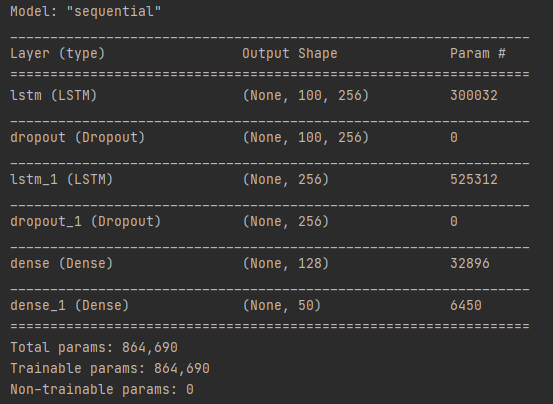
\includegraphics[scale=.6]{modelli/modello_buono.png}
		\caption{\label{fig:best_mod}Summary of the best model.}
	\end{figure}
	
	\null
	\vfill